\documentclass[11pt,fleqn]{article}

\usepackage[latin1]{inputenc}
\usepackage{enumerate}
\usepackage[hang,flushmargin]{footmisc}
\usepackage{amsmath}
\usepackage{amsfonts}
\usepackage{amssymb}
\usepackage{amsthm}
\usepackage{graphicx}
\graphicspath{ {images/} }

\theoremstyle{definition}
\newtheorem{theorem}{Theorem}
\newtheorem{lemma}[theorem]{Lemma}
\newtheorem{corollary}[theorem]{Corollary}
\newtheorem{proposition}[theorem]{Proposition}
\newtheorem{definition}[theorem]{Definition}
\newtheorem{example}[theorem]{Example}

\setlength{\oddsidemargin}{0px}
\setlength{\textwidth}{460px}
\setlength{\voffset}{-1.5cm}
\setlength{\textheight}{20cm}
\setlength{\parindent}{0px}
\setlength{\parskip}{10pt}

\begin{document}
\begin{center}
{\Huge
Installation of Android Tools
}\\
\end{center}

Please make sure that you follow all of these instructions and that you have
everything ready for the next class.

\begin{enumerate}[1.]
\item
Download and install the Java 7 JDK from here:\newline
http://www.oracle.com/technetwork/java/javase/downloads/jdk7-downloads-1880260.html

\item
Download the ftc library and app from the following link:\newline
https://goo.gl/0DxzY\newline
You can find the download link in the bottom right where is says ``Download
link". Once you download the file, unzip it and then move it to where you would
like to keep the project. 

\begin{center}
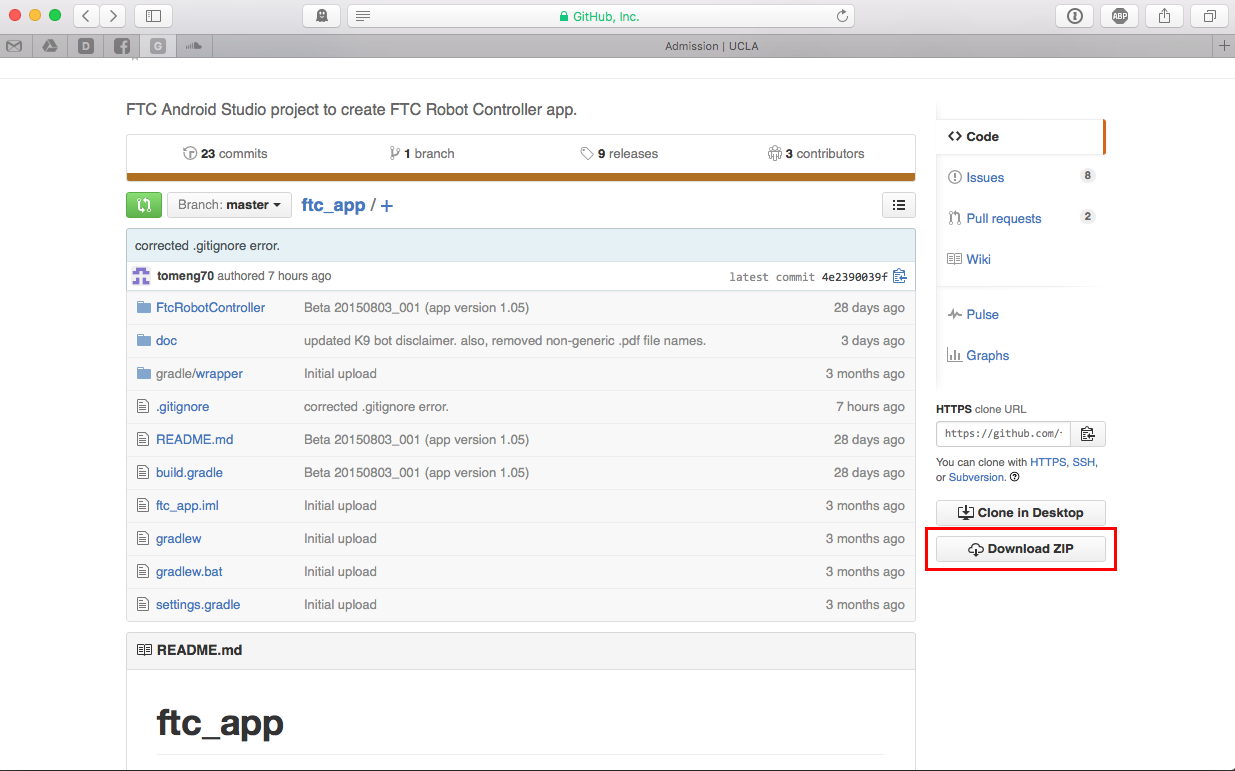
\includegraphics[scale=.3]{Step1}
\end{center}

\item
Open Android Studio. On the welcome screen, there should be an option
``Configure". Click this option and then the first option on the next screen
should be ``SDK Manager". Open the SDK Manager. 

\begin{center}
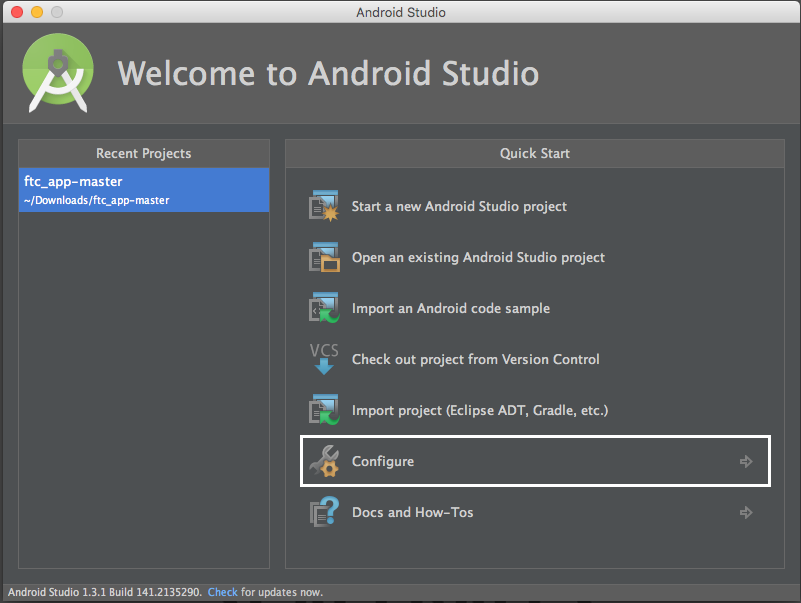
\includegraphics[scale=.3]{Step2}
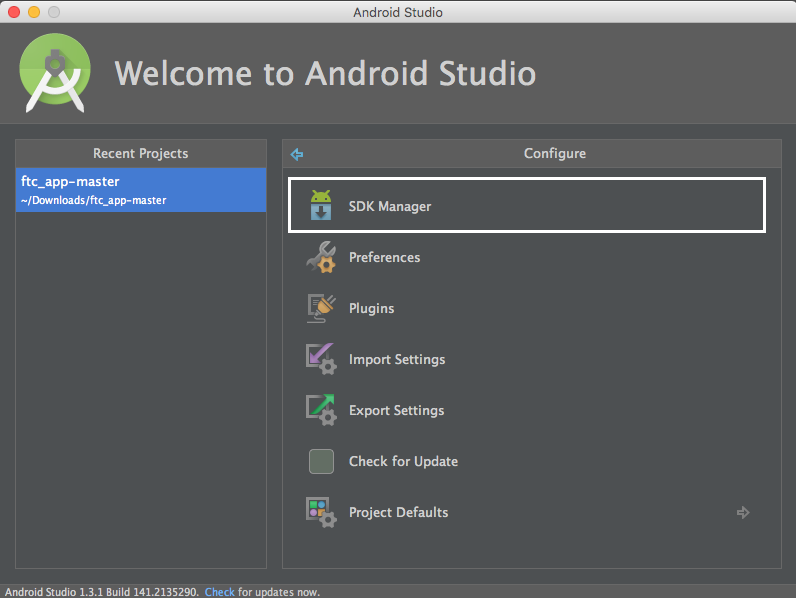
\includegraphics[scale=.3]{Step3}
\end{center}

\item
There is an option on the bottom of the SDK Manager that says ``deselect all".
Pick this option. Scroll down to API 19. There should be a checkbox right next
to the API 19 option. Click this box and follow the prompts to install the API. 

\begin{center}
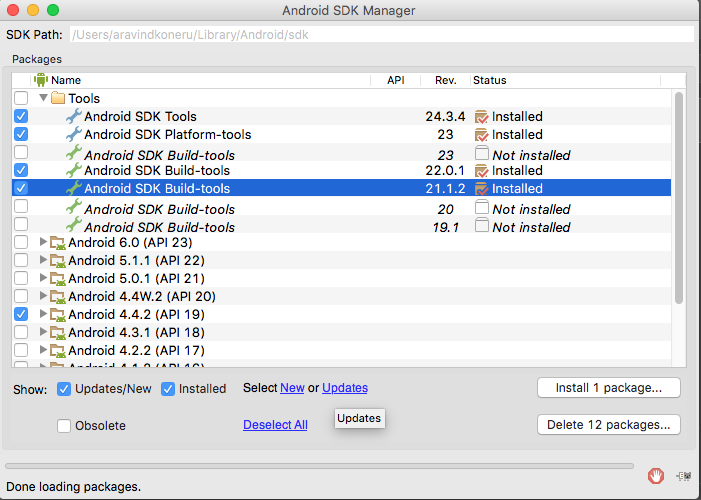
\includegraphics[scale=.3]{Step4}
\end{center}

\item
Wait for the download to finish and then restart Android Studio. 

\item
You should see an option that says ``Import Project". Click this option and go
the FTC app folder you downloaded in step 2. Choose the \texttt{build.gradle}
file and open it. 

\begin{center}
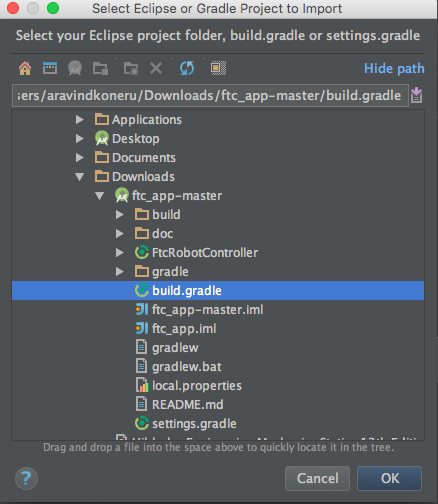
\includegraphics[scale=.3]{Step5}
\end{center}

\item
Wait approx. 30 seconds and then look at the bottom left  of Android Studio. You
should see some text that says ``Grade bundle finished" with a time. This means
that you have successfully configured and installed the Android API and the
FIRST SDK. 
\end{enumerate}

\end{document}
